\documentclass[8pt,a4paper]{article}
\usepackage{graphicx}
\usepackage{amsmath}
\usepackage{amsfonts}
\usepackage{amssymb,amsthm}
\usepackage{array}
\usepackage{setspace}
\spacing{0.75}
\usepackage[spanish, activeacute]{babel} %Definir idioma español
\usepackage[utf8]{inputenc} 

\voffset 0 cm \hoffset 0 cm \addtolength{\textwidth}{0cm}
\addtolength{\textheight}{0cm}\addtolength{\leftmargin}{0cm}

\begin{document}
%style file for ESANN manuscripts
\title{Procesamiento de texto manuscrito usando conjuntos de clasificadores}

%***********************************************************************
% AUTHORS INFORMATION AREA
%***********************************************************************
\author{
Emilio Samuel Aced Fuentes \\
Roberto Alcober Couso \\
Arturo Bl\'azquez P\'erez \\
Nicol\'as Trejo Moya \\
}
%***********************************************************************
% END OF AUTHORS INFORMATION AREA
%***********************************************************************

\maketitle

\section{Introducci\'on}
En este proyecto vamos a clasificar im\'agenes de letras manuscritas intentando predecir de forma correcta el s\'imbolo que representan.
Utilizaremos varios algoritmos de clasificaci\'on y los compararemos para encontrar los mejores resultados posibles, viendo diferencias de tiempos y  tasa de acierto.


\section{An\'alisis de los datos}
En el dataset provisto, est\'an representadaslas 10 primeras letras del alfabeto(A-J), por tanto 10 clases las cuales hemos etiquetado en nuestra base de datos etiquetadas de 0 a 10 respectivamente.
Las imagenes nos vienen en un tamaño de $206\times150$ en escala de grises.


\begin{figure}[htbp]
	\centering
    \includegraphics[scale=0.5]{./sin_procesar/l00000_A.png}
    \caption{Ejemplo de una A}
\end{figure}



Como podemos observar las imagenes contienen ruido, el cual podría dificultar la tarea de clasificación gravemente.Este problema lo hemos solucionado sometiendo a la imagen a diferentes tratamientos.

\subsection{Tratamientos}

Para todos los experimentos de este proyecto hemos umbralizado la imágen mediante otsu y posteriormente hemos realizado un filtro de mediana con un kernel cuadrado de tamaño 3.
Esto nos ha dado el siguiente resultado:
\begin{figure}[htbp]
	\centering
    \includegraphics[scale=0.5]{./procesado/l00000_A.png}
    \caption{Ejemplo de una A tratada}
\end{figure}

A continuación explicaremos los tratamientos que le hemos aplicado a las imágenes para reducir la complejidad del problema

\subsection{Atributos}
Teniendo en cuenta que las imágenes son matrices $206\times150$ lo cual nos da un total de 30900 atributos, lo cual es una cantidad de atributos desorbitada, por ese motivo hemos decidido ver como afecta reducir la dimensión.
Las principales modificaciones que realizaremos a las imagenes para reducir su dimensionalidad son las siguientes:

\paragraph{Eliminar filas y columnas poco importantes}


Esto lo realizaremos mediante la selección de un umbral, con el cual consideraremos que las filas y columnas que tengan una cantidad menor de zona pintada que el umbral especificado no son de relevancia y por tanto las despreciaremos del problema

\begin{figure}[htbp]
    \centering
    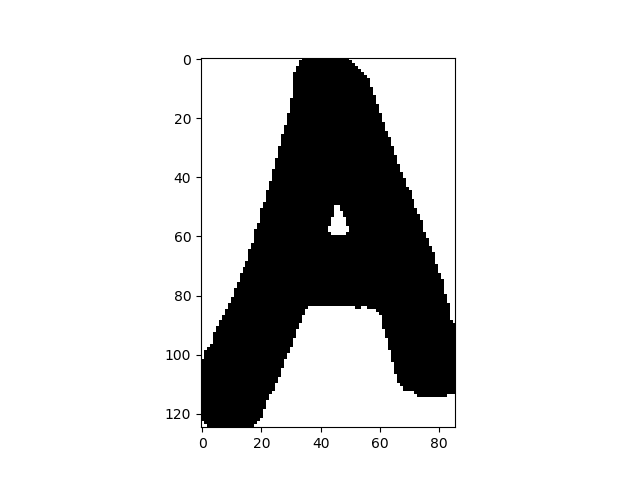
\includegraphics[scale=0.5]{./Arecortada.png}
    \caption{Ejemplo de una A recortada}
\end{figure}

\paragraph{Redimensionar la imágen interpolando}

Con el fin de evitar el aliasing (meter bordes que no existian al reducir una imágen) hemos redimensionado la imágen siempre aplicando un kernel gausiano previamente.

A continuacion mostraremos distintos valores de los tamaños de las imágenes que compararemos en nuestro estudio:

\begin{figure}[htbp]
   \centering
    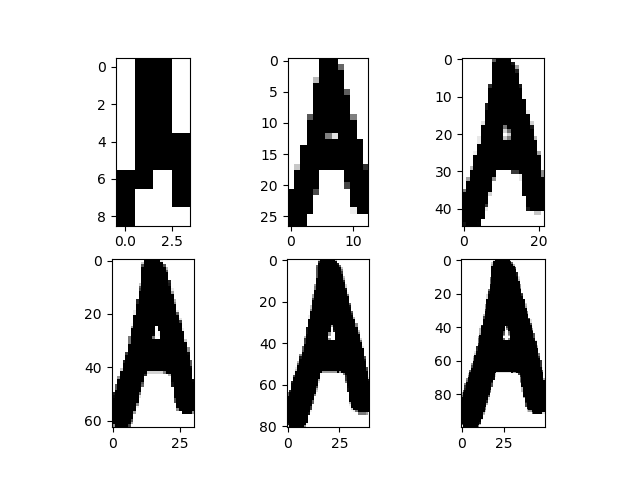
\includegraphics[scale=0.5]{./A_Variando_Tam.png}
    \caption{Varios tamaños de una A que usaremos}
\end{figure}


\section{Modelos}

Usaremos los siguientes clasificadores en este trabajo:
\begin{enumerate}
\item Random Forest
\item SVC
\item KNN
\end{enumerate}
en los cuales variaremos los tamaños de las imágenes y compararemos tiempos y tasa de aciertos para poder decidirnos por uno.

Para todos ellos destinaremos la mitad de los datos para train y la otra mitad para test.

\subsection{Random Forest}

Con random forest hemos encontrado que funciona muy bien incluso reduciendo mucho la dimension de los datos encontrando que la mejor tasa de acierto comparandola con el tiempo es reducir las imagenes a cuadrados $9\times4$ con 500 arboles de profundidad máxima 10 consiguiendo los siguientes resultados:
\begin{enumerate}
\item \textbf{Tasa de acierto}: 92.57$\%$
\item \textbf{Matriz de confusion}:
	
\[
M=
  \begin{bmatrix}
    69 & 1 & 0 & 0 & 0 & 0 & 0 & 0 & 0 & 0 \\
    2 & 48 & 0 & 5 & 2 & 3 & 0 & 0 & 4 & 0 \\
    0 & 0 & 73 & 0 & 0 & 0 & 1 & 0 & 0 & 0 \\
    0 & 3 & 0 & 59 & 0 & 2 & 0 & 0 & 0 & 0 \\
    0 & 1 & 1 & 0 & 54 & 1 & 1 & 0 & 1 & 0 \\
    0 & 0 & 0 & 0 & 1 & 61 & 0 & 0 & 0 & 0 \\
    0 & 1 & 0 & 0 & 0 & 1 & 66 & 0 & 0 & 0 \\
    2 & 2 & 0 & 0 & 0 & 0 & 0 & 67 & 1 & 0 \\
    1 & 0 & 1 & 1 & 0 & 0 & 1 & 0 & 58 & 6 \\
    0 & 0 & 0 & 0 & 0 & 1 & 0 & 0 & 2 & 56 \\
  \end{bmatrix}
\]

\item \textbf{Ejemplos de clasificacion}

\begin{figure}[htbp]
    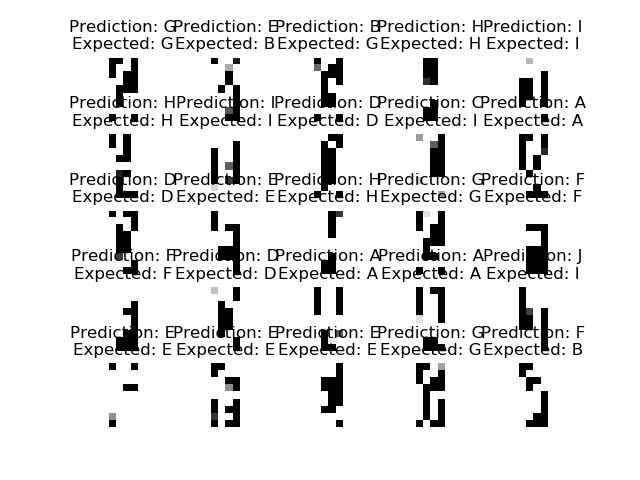
\includegraphics[scale=0.5]{./RandomForest_9_4.png}
    \caption{Ejemplos de clasificacion con random forest}
\end{figure}
\end{enumerate}

\subsection{Clasificador SVC}

Es el algoritmo que más tarda de los 3 con los que hemos experimentado, pero a su vez es el que consigue la mejor tasa de acierto. Para el ánalisis de resultados de este clasificador con estos datos decidimos reducir las imagenes a $100\times50$ con una gamma de 0.001 obteniendo los siguientes resultados:
\begin{enumerate}
\item \textbf{Tasa de acierto}: 96.21$\%$
\item \textbf{Matriz de confusion}:
	
\[
M=
  \begin{bmatrix}
    69 & 1 & 0 & 0 & 0 & 0 & 0 & 0 & 0 & 0 \\
    1 & 57 & 0 & 3 & 0 & 3 & 0 & 0 & 0 & 0 \\
    0 & 0 & 74 & 0 & 0 & 0 & 0 & 0 & 0 & 0 \\
    1 & 1 & 0 & 62 & 0 & 0 & 0 & 0 & 0 & 0 \\
    0 & 1 & 0 & 0 & 57 & 1 & 1 & 0 & 0 & 0 \\
    0 & 0 & 0 & 0 & 0 & 62 & 0 & 0 & 0 & 0 \\
    0 & 0 & 1 & 0 & 0 & 1 & 66 & 0 & 0 & 0 \\
    1 & 0 & 0 & 1 & 0 & 0 & 0 & 70 & 0 & 0 \\
    0 & 0 & 0 & 0 & 2 & 0 & 0 & 0 & 61 & 5 \\
    0 & 0 & 0 & 0 & 0 & 0 & 0 & 0 & 2 & 57 \\
  \end{bmatrix}
\]

\item \textbf{Ejemplos de clasificacion}

\begin{figure}[htbp]
    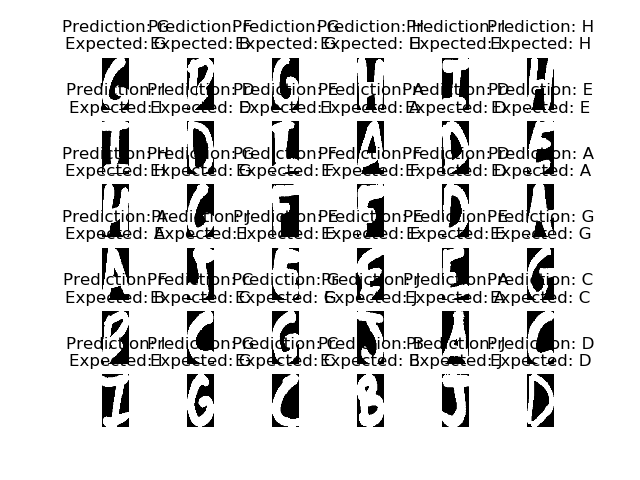
\includegraphics[scale=0.5]{./SVC100_50.png}
    \caption{Ejemplos de clasificacion con SVC}
\end{figure}
\end{enumerate}


\subsection{Clasificador KNN}

Como podremos ver más adelante este es un clasificador con el que conseguimos unos resultados medios, no tarda tanto como SVC ni tiene una tasa de acierto tan grande con imágenes tan reducidas como random forest pero aún así funcionó nos pareció suficientemente bueno como para incluirlo en la memoria
\begin{enumerate}
\item \textbf{Tasa de acierto}: 94.39$\%$
\item \textbf{Matriz de confusion}:
	
\[
M=
  \begin{bmatrix}
    69 & 1 & 0 & 0 & 0 & 0 & 0 & 0 & 0 & 0 \\
    1 & 53 & 0 & 2 & 0 & 3 & 0 & 0 & 5 & 0 \\
    0 & 0 & 74 & 0 & 0 & 0 & 0 & 0 & 0 & 0 \\
    1 & 1 & 0 & 61 & 0 & 0 & 0 & 0 & 1 & 0 \\
    0 & 0 & 2 & 0 & 52 & 2 & 1 & 0 & 2 & 0 \\
    0 & 0 & 0 & 0 & 0 & 62 & 0 & 0 & 0 & 0 \\
    0 & 0 & 5 & 0 & 0 & 1 & 62 & 0 & 0 & 0 \\
    0 & 0 & 0 & 0 & 0 & 0 & 0 & 71 & 1 & 0 \\
    0 & 1 & 0 & 0 & 1 & 0 & 0 & 0 & 62 & 4 \\
    0 & 0 & 0 & 0 & 0 & 0 & 0 & 0 & 2 & 57 \\
  \end{bmatrix}
\]

\item \textbf{Ejemplos de clasificacion}

\begin{figure}[htbp]
\centering
    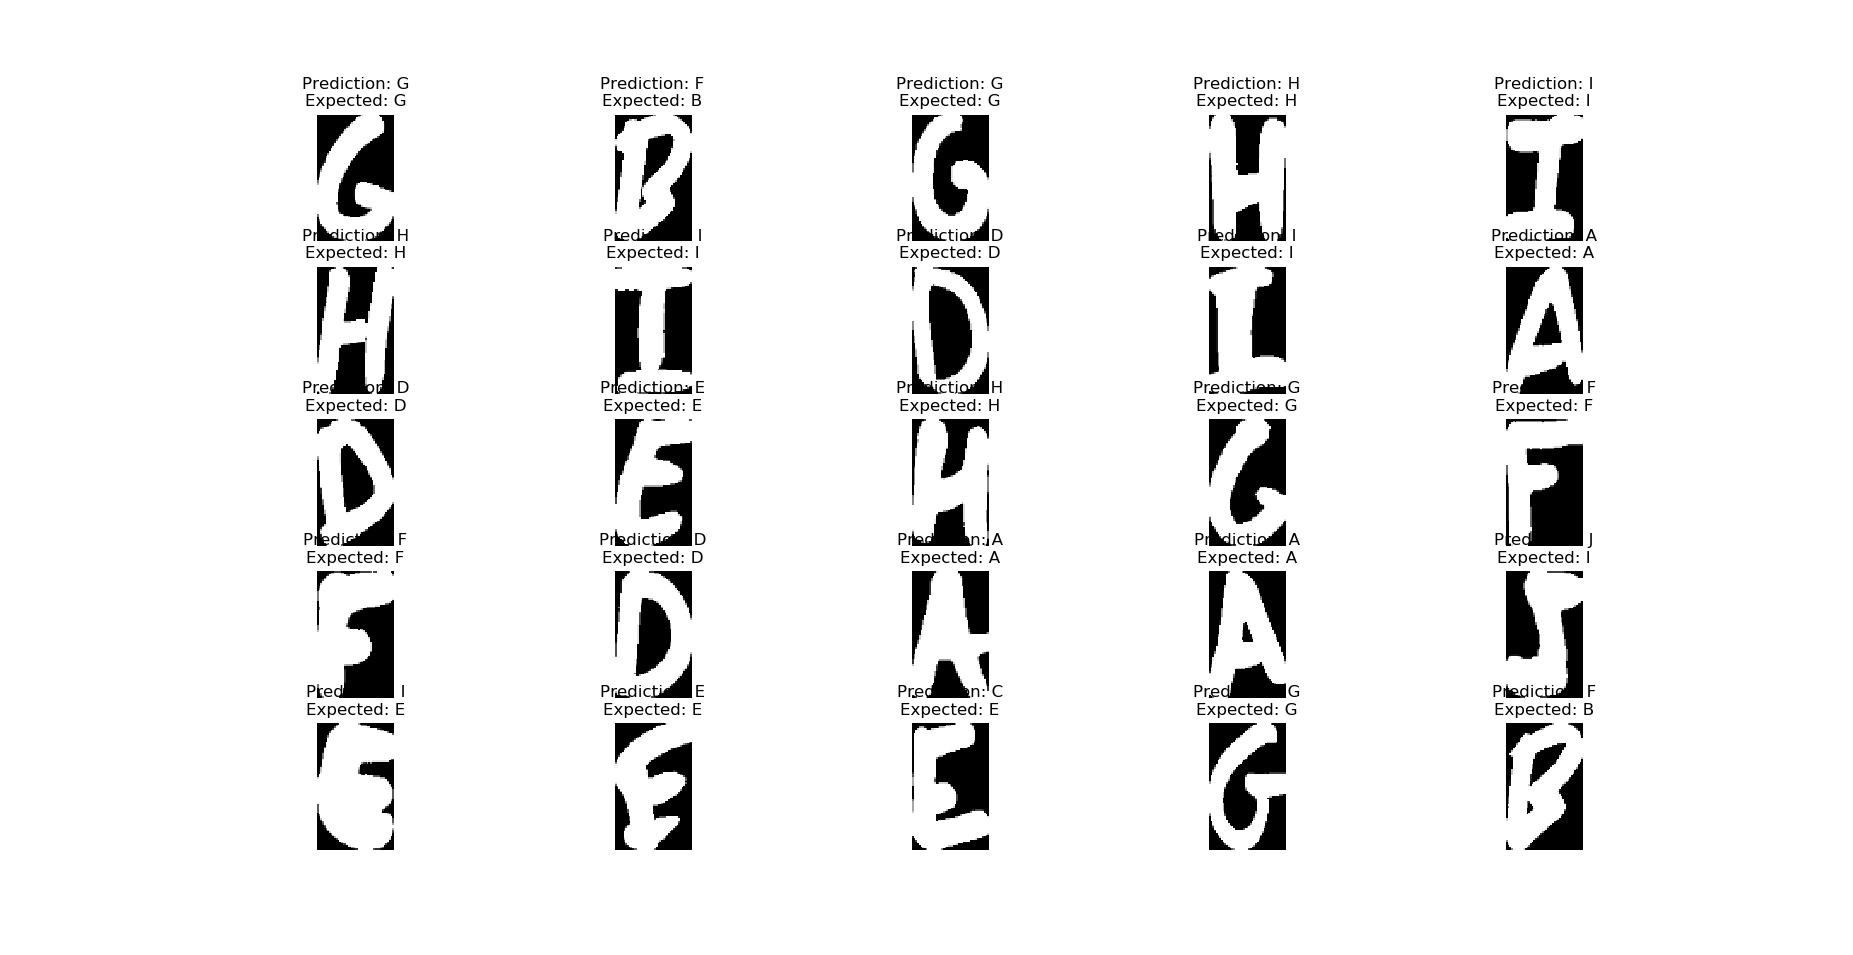
\includegraphics[scale=0.5]{./KNN_Ejemplos.png}
    \caption{Ejemplos de clasificacion con KNN}
\end{figure}
\end{enumerate}

\subsection{Comparar los clasificadores por su tasa de acierto}

Hemos decidido ir variando el número de parámetros que consideramos para ver como esto afecta tanto al tiempo de clasificacion como a la tasa de aciertos:
\begin{figure}[htbp]
    \centering
    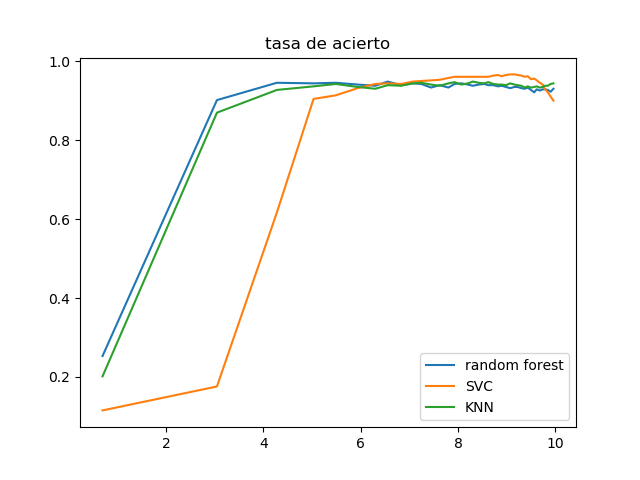
\includegraphics[scale=0.05]{./CompararAciertos.png}
    \caption{Comparar las tasas de acierto con los 3 clasificadores}
\end{figure}

En esta figura muestra en el eje de las x la dimensión de los datos que usamos para clasificar en escala logaritmica y en el eje y la tasa de acierto.
Como podemos ver a medida que aumentamos la cantidad de datos a usar SVC aumenta su tasa de acierto alcanzando un máximo con imágenes de tamaño $100\times50$, pero al contrario que con KNN y random forest, vemos que cuando empezamos a interpolar y a hacer las imágenes más grandes que el tamaño original su tasa baja.
Miremos aumentando más aún el tamaño de las imágenes:
\begin{figure}[htbp]
    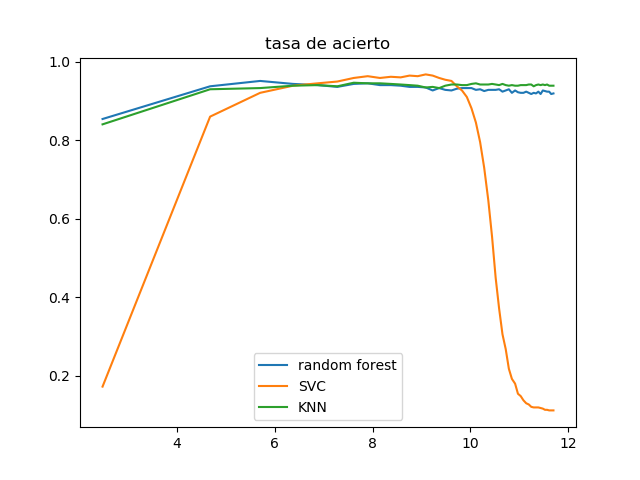
\includegraphics[scale=0.5]{./AciertosFinal.png}
    \caption{Comparar las tasas de acierto con los 3 clasificadores}
\end{figure}
Como podemos ver su rendimiento baja notablemente, por eso concluimos en que SVC es menos robusto que KNN y Random Forest

\subsection{Comparar los clasificadores por su tiempo de ejecución}

En este apartado compararemos los tiempos de construir el clasificador y clasificar de KNN, SVC y Random Forest.

\begin{figure}[htbp]
    \centering
    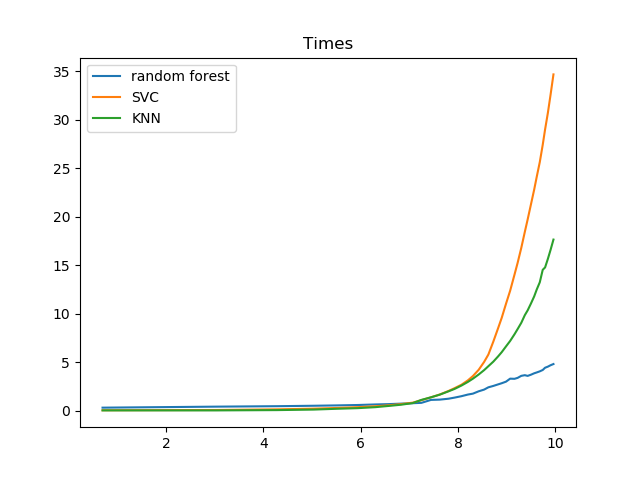
\includegraphics[scale=0.5]{./CompararTiempos.png}
    \caption{Comparar los tiempos de ejecucion con los 3 clasificadores}
\end{figure}

Como podemos ver en la figura 10 la diferencia entre los tiempos de ejecución en el limite son bastante notables encontrando que SVC es el más lento seguido de KNN y Random Forest el más rápido.

A continuación compararemos el tiempo que tardan con su tasa de acierto, con el objetivo de poder comparar para un limite de tiempo dado cual es mejor:
\begin{figure}[htbp]
    \centering
    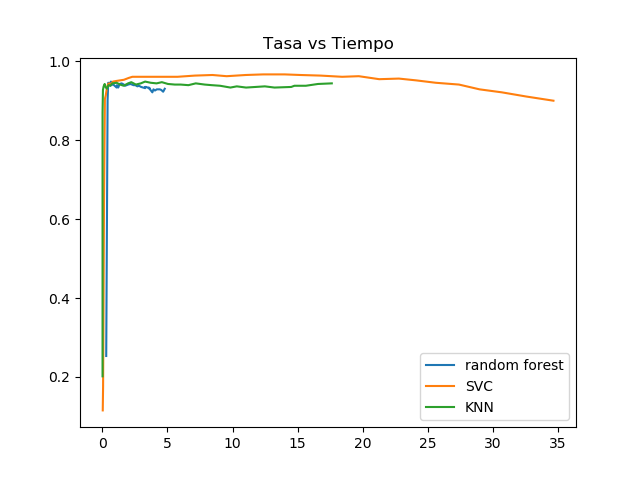
\includegraphics[scale=0.5]{./CompararAciertosvsTiempos.png}
    \caption{Comparar las tasas de acierto vs su tiempo de ejecucion con los 3 clasificadores}
\end{figure}

Finalmente compararemos solamente el tiempo de clasificación sin contar el tiempo de construir el clasificador.

\end{document}
